%!TEX root = ../../report.tex

\begin{figure}[H]
	\newcommand{\figurewidth}{0.5\textwidth}
	\begin{subfigure}[b]{\figurewidth}
        \figureborder{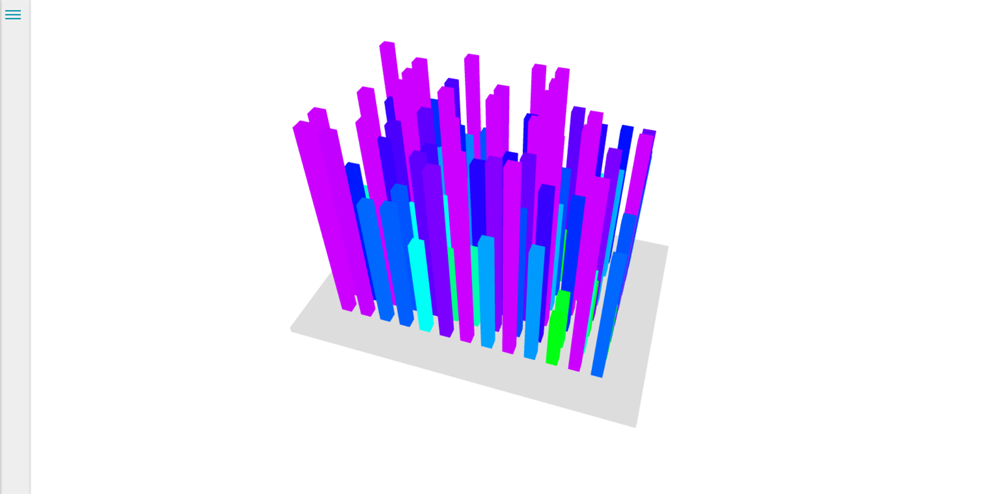
\includegraphics[width=\textwidth]{images/implementation/drawer/closed}}
		\caption{Closed drawer.}
		\label{fig:closed_drawer}
	\end{subfigure}
	\begin{subfigure}[b]{\figurewidth}
		\figureborder{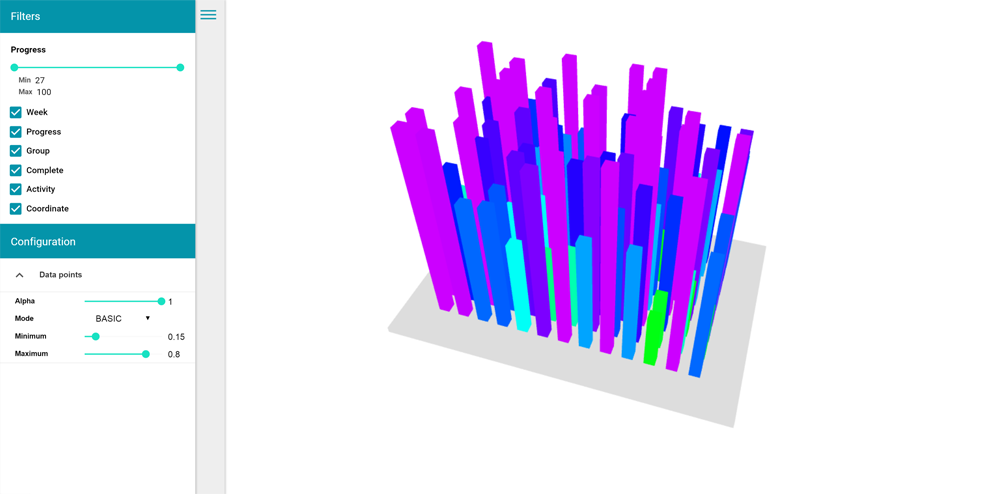
\includegraphics[width=\textwidth]{images/implementation/drawer/open}}
		\caption{Open drawer.}
		\label{fig:open_drawer}
	\end{subfigure}
	\caption{Drawer interface.}
	\label{fig:drawer}
\end{figure}
